\section{Approximating Area}
\label{sec:area-approx}
% From Section 3.1.
\subsection{PreCalculus Idea – The Area of a Rectangle}
If you look on the inside cover of nearly any traditional math book, you will find a bunch of area and volume formulas – the area of a square, the area of a trapezoid, the volume of a right circular cone, and so on. Some of these formulas are pretty complicated. But you still won't find a formula for the area of a jigsaw puzzle piece or the volume of an egg. There are lots of things for which there is no formula. Yet we might still want to find their areas.

One reason areas are so useful is that they can represent quantities other than simple geometric shapes. If the units for each side of the rectangle are meters, then the area will have the units meters$\times$meters = square meters = m$^2$. But if the units of the base of a rectangle are hours and the units of the height are miles/hour, then the units of the area of the rectangle are hours$\times$miles/hour = miles, a measure of distance. Similarly, if the base units are centimeters and the height units are grams, then the area units are gram-centimeters, a measure of work.

\begin{figure}[!ht]
  \centering
    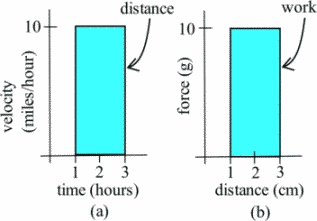
\includegraphics[width=0.4\textwidth]{img/chap5/image065.png}
    \caption{Modeling distance traveled and work with rectangles}
    \label{fig:5-2-rectangles}
\end{figure}
The basic shape we will use is the rectangle; the area of a rectangle is base$\times$height. You should also know the area formulas for triangles: $A=\dfrac{1}{2}bh$, and for circles: $A=\pi r^2$.

%Section 3.1: The Definite Integral
\subsection{Distance from Velocity}
\begin{example}
Suppose a car travels on a straight road at a constant speed of 40 miles per hour for two hours. See the graph of its velocity in Figure \ref{fig:5-2-distance}. How far has it gone?

\begin{figure}[!ht]
  \centering
    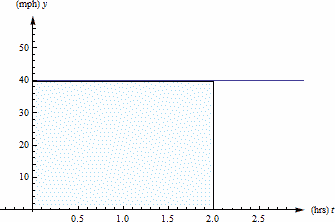
\includegraphics[width=0.4\textwidth]{img/chap5/image001.png}
    \caption{Car velocity as a function of time.}
    \label{fig:5-2-distance}
\end{figure}
\begin{solution}
We all remember distance = rate$\times$time, so this one is easy. The car has gone (40 miles/hour)$\times$(2 hours) = 80 miles.
\end{solution}\end{example}

\begin{example}
Now suppose that a car travels so that its speed increases steadily from 0 to 40 miles per hour, for two hours. (Just be grateful you weren’t stuck behind this car on the highway.) See the graph of its velocity in below. How far has this car gone?

\begin{figure}[!ht]
  \centering
    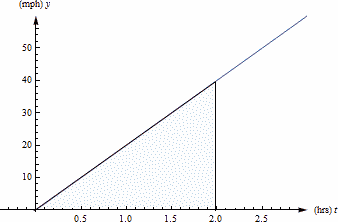
\includegraphics[width=0.4\textwidth]{img/chap5/image002.png}
    \caption{Car velocity as a function of time.}
    \label{fig:5-2-distance2}
\end{figure}

\begin{solution}
The trouble with our old reliable distance = rate$\times$time relationship is that it only works if the rate is constant. If the rate is changing, there isn’t a good way to use this formula.

But look at the graph from the last example again. Notice that distance = rate$\times$time also describes the area between the velocity graph and the $t$-axis, between $t=0$ and $t=2$ hours. The rate is the height of the rectangle, the time is the length of the rectangle, and the distance is the area of the rectangle. This is the way we can extend our simple formula to handle more complicated velocities: And this is the way we can answer the second example.

The distance the car travels is the area between its velocity graph, the $t$-axis, $t=0$ and $t=2$. This region is a triangle, so its area is
$$\frac{1}{2}bh = \frac{1}{2}(2 \text{ hours})(40 \text{ miles per hour}) = 40 \text{ miles}\enspace .$$
So the car travels 40 miles during its annoying trip.
\end{solution}\end{example}

In our distance/velocity examples, the function represented a rate of travel (miles per hour), and the area represented the total distance traveled. This principle works more generally.

For functions representing other rates such as the production of a factory (bicycles per day), or the flow of water in a river (gallons per minute) or traffic over a bridge (cars per minute), or the spread of a disease (newly sick people per week), the area will still represent the total amount of something.

graph
\begin{example}
The graph below shows the flow rate (cubic feet per second) of water in the Skykomish river at the town of Goldbar in Washington state.

graph
\begin{solution}
The area of the shaded region represents the total volume (cubic feet or ft$^3$) of water flowing past the town during the month of October. We can approximate this area to approximate the total water by thinking of the shaded region as a rectangle with a triangle on top.
\begin{align*}
\text{Total water} &= \text{total area} \\
  &\approx \text{area of rectangle} + \text{area of the ``triangle''}\\
  &\approx  \left(2000 \frac{\text{ft}^3}{\text{s}}\right)(30 \text{days})+12\left(1500\frac{\text{ft}^3}{\text{s}}\right)(30 \text{days})\\
  &= \left(2570 \frac{\text{ft}^3}{\text{s}}\right)(30 \text{days})
\end{align*}
Note that we need to convert the units to make sense of our result:
\begin{align*}
\text{Total water} &\approx  \left(2570 \frac{\text{ft}^3}{\text{s}}\right)(30 \text{days}) \\
  &=\left(2570 \frac{\text{ft}^3}{\text{s}}\right)(2592000 \text{s}) \\
  &\approx 7.128 \cdot 10^9 \text{ft}^3
\end{align*}
About 7 billion cubic feet of water flowed past Goldbar in October.
\end{solution}\end{example}

\subsection{Approximating with Rectangles}
How do we approximate the area if the rate curve is, well, curvy? We could use rectangles and triangles, like we did in the last example. But it turns out to be more useful (and easier) to simply use rectangles. The more rectangles we use, the better our approximation is.

graph
Suppose we want to calculate the area between the graph of a positive function $f(x)$ and the $x$-axis on the interval $[a,b]$ (graphed above). The {\bf Riemann Sum method}\index{Riemann sum} builds several rectangles with bases on the interval $[a,b]$ and sides that reach up to the graph of $f(x)$ (see below). Then the areas of the rectangles can be calculated and added together to get a number called a {\bf Riemann Sum} of $f$ on $[a,b]$. The area of the region formed by the rectangles is an approximation of the area we want.

graph
\begin{example}
Approximate the area in the graph on the left between the graph of $f$ and the $x$-axis on the interval $[2, 5]$ by adding the areas of the rectangles in the graph on the right.

graph
\begin{solution}
The total area of rectangles is
$$(2)(3)+(1)(5)=11 \enspace .$$
\end{solution}\end{example}

\begin{example}
Let A be the region bounded by the graph of $f(x)=\frac{1}{x}$, the $x$-axis, and vertical lines at $x=1$ and $x=5$. We can’t find the area exactly (with what we know now), but we can approximate it using rectangles.

\begin{solution}
When we make our rectangles, we have a lot of choices. We could pick any (non-overlapping) rectangles whose bottoms lie within the interval on the $x$-axis, and whose tops intersect with the curve somewhere. But it is easiest to choose rectangles that (a) have all the same width and (b) take their heights from the function at one edge. Below are graphs showing two ways to use four rectangles to approximate this area. In the first graph, we used left-endpoints; the height of each rectangle comes from the function value at its left edge. In the second graph on the next page, we used right-hand endpoints.

\paragraph{Left-hand endpoints:} The area is approximately the sum of the areas of the rectangles. Each rectangle gets its height from the function $f(x)=\frac{1}{x}$ and each rectangle has a width of 1.

graph
You can find the area of each rectangle using area = height$\times$width. So the total area of the rectangles, the left-hand estimate of the area under the curve, is
$$f(1) \cdot 1 + f(2) \cdot 1 + f(3) \cdot 1 + f(4) \cdot 1 = 1 + \frac{1}{2} + \frac{1}{3} + \frac{1}{4} = \frac{25}{12}\approx   2.08 \enspace .$$
Notice that because this function is decreasing, all the left endpoint rectangles stick out above the region we want – using left-hand endpoints will overestimate the area.

\paragraph{Right-hand endpoints:} The right-hand estimate of the area is
$$f(2) \cdot 1 + f(3) \cdot 1 + f(4) \cdot 1 + f(5) \cdot 1 = \frac{1}{2} + \frac{1}{3} + \frac{1}{4} + \frac{1}{5} = \frac{77}{60} \approx   1.28 \enspace .$$
graph
All the right-hand rectangles lie completely under the curve, so this estimate will be an underestimate.

We can see that the true area is actually in between these two estimates. So we could take their average:
$$\text{Average} = \dfrac{\frac{25}{12} + \frac{77}{60}}{2} = \frac{101}{60}\approx   1.68 \enspace .$$
In general, the average of the left-hand and right-hand estimates will be closer to the real area than either individual estimate.

Our estimate of the area under the curve is about 1.68. (The actual area is about 1.61.)

%This applet will allow you to see how the approximation changes if you use more rectangles; change the position slider to switch between using the left endpoints, right endpoints, and midpoints:
\end{solution}\end{example}


If we wanted a more accurate solution, we could use even more and even narrower rectangles. But there is a limit to how much work we want to do by hand. In practice, choose a manageable number of rectangles. We will have better methods to get more accurate answers before long.

These sums of areas of rectangles are called {\bf Riemann sums}\index{Riemann sum}. You may see a shorthand notation used when people talk about sums. We won't use it much in this book, but you should know what it means.

\begin{definition}[Riemann Sum]
A Riemann sum of a function $f(x)$ over an interval $[a,b]$ is a sum of areas of rectangles that approximates the area under the curve. Start by dividing the interval $[a,b]$ into $n$ subintervals; each subinterval will be the base of one rectangle. We usually make all the rectangles the same width $\Delta x$. The height of each rectangle comes from the function evaluated at some point in its sub interval. Then the Riemann sum is
$$f(x_1)\Delta x + f(x_2)\Delta x+f(x_3)\Delta x + \ldots +f(x_n)\Delta x$$
or, factoring out the $\Delta x$,
$$\Delta x(f(x_1)+f(x_2)+f(x_3)+\ldots +f(x_n)) \enspace .$$
\end{definition}
\begin{definition}[Sigma Notation\index{Sigma notation}]
The upper-case Greek letter Sigma $\Sigma$ is used to stand for sum. {\bf Sigma notation} is a way to compactly represent a long, infinite, or arbitrarily long sum of many similar terms, such as a Riemann sum.

Using the Sigma notation, the Riemann sum can be written
$$\sum_{i=1}^n f(x_i)\Delta x \enspace .$$
This is read aloud as ``the sum as $i$ goes from 1 to $n$ of $f$ of $x$ sub $i$ times $\Delta x$.'' The $i$ is a {\bf counter}\index{Counter} or {\bf index}\index{Index}, like you might have seen in a programming class. The index increases by 1 each term and must always be an integer.
\end{definition}

% \subsection{Approximating with Technology}
% If your function is given as a graph or table, you will still have to approximate definite integrals using areas, usually of rectangles. But if your function is given as a formula, you can turn to technology to get a better approximate answer. For example, most graphing calculators have some kind of numerical integration tool built in. You can also find many online tools that can do this; type numerical integration into any search engine to see a selection of these.
%
% Most numerical integration tools use rectangles to estimate the signed area, just as you would do by hand. But they use many more rectangles than you would have the patience for, so they get a better answer. Some of them use computer algebra systems to find exact answers; we will learn how to do this ourselves later in this chapter.
%
% When you turn to technology to find the value of a definite integral, be careful. Not every tool will be able to give you a correct answer for every integral. You should make an estimate of the answer yourself first so you can judge whether the answer you get makes sense.
%
% \begin{example}
% Use technology to approximate the area under the curve $y=\dfrac{1}{x}$ over the interval $[1, 5]$. (This is the same area we approximated with rectangles before.)
%
% \begin{solution}
% We could use the following command in GeoGebra to approximate this integral:
%
% Integral[1 / x, 1, 5]
% Or click this link to see how to evaluate this integral using Wolfram|Alpha.
% \end{solution}\end{example}
%
% \begin{example}
% Use technology to approximate the area under he curve $y = e^{x^2+x}$ over he interval $[1, 2]$.
%
% \begin{solution}
%   The function here is positive, so there must be some area under the curve here. There isn’t an algebraic way to find the exact answer, so some programs may just return the original integral rather than try to approximate it.
%
% We could use the following command in GeoGebra to approximate this integral:
%
% Integral[e^(x^2 + x), 1, 2]
% Or click this link to see how to approximate this integral using Wolfram|Alpha. Although it looks like Wolfram|Alpha can evaluate the integral, the Erfi function that it shows in its answer is actually defined in terms of another integral, so it still hasn't found an algebraic answer.
% \end{solution}\end{example}

% Exercize: Example () gives an example of when a left Riemann sum underestiamted the area and the right Riemann sum overestimated area. Give an example of when a left Riemann sum overestimates the area and a right Riemann sum underestimates the area.
